%!TEX root=../../sbc-template.tex
%% Ideia global da seção
% O que é Deep Learning?
% Quais as características das Redes Neurais Convolucionais?

O Aprendizado de Máquina (AM) é uma sub-área da Inteligência Artificial que lida com algoritmos que são melhorados de forma implícita a partir de exemplos do domínio considerado \cite{Faceli:Livro}. A maioria dos problemas abordados com modelos, métodos e técnicas dessa área compreendem tarefas complexas cuja solução analítica por meio dos algoritmos tradicionais é inviável ou até mesmo impraticável \cite{Brink:MachineLearningLivro}.

No contexto de AM, ``aprender'' é um termo que denota o processo de busca automática pela melhor representação da informação que viabiliza a transformação dos dados de entrada com o intuito de facilitar a resolução de uma dada tarefa considerada, a exemplo de uma classificação binária \cite{Chollet:2017}. Para efetuar essa busca automática, entretanto, faz-se necessária a intervenção humana altamente especializada para escolha dos melhores modelos, parâmetros e hiper-parâmetros, os quais são diretamente relacionados ao sucesso na resolução da tarefa considerada \cite{Khan:2018}.

Com o intuito de tornar o processo de aprendizado mais independente, \emph{Deep Learning} (DL), uma sub-área de AM, têm se destacado em diversos contextos práticos, pois objetiva aprender automaticamente, por meio de diversas camadas hierárquicas e sucessivas, múltiplas representações complexas de dados de entrada multimodais (imagens, sons, vídeo, etc.), aumentado assim o domínio de problemas que podem ser abordados \cite{Buduma:2018}. Para o domínio de DL, as CNNs são o modelo de referência para múltiplas tarefas. As mesmas são um tipo recente de Rede Neural Artificial \emph{Feedforward Multilayer Perceptron} (RNA MLP), as quais compõem o paradigma conexionista da Inteligência Artificial \cite{Russel:IABiblia}. As RNAs MLP são compostas por um conjunto de unidades básicas de processamento, denominadas neurônios artificiais, que são fortemente interconectados e organizados segundo camadas, operando nos dados de entrada com o objetivo de inferir uma função que aprenda as respectivas saídas, conforme o paradigma de Aprendizado Supervisionado \cite{Khan:2018}.

Os neurônios artificiais são inspirados nos neurônios biológicos e funcionam de forma independente como unidades computacionais simples que recebem sinais de entrada e atribui-lhes pesos, produzindo um sinal de saída usando uma função de ativação. A Figura \ref{fig:neuronio} ilustra a estrutura de um neurônio abstrato com $n$ entradas, em que cada canal de entrada é um valor $x_i \in \mathbbm{R}$. Cada entrada possui um peso associado $w_i \in \mathbbm{R}$, e o corpo do neurônio calcula a soma ponderada das entradas e sujeita esse valor a uma função de ativação $f(\cdot)$, que define o limite no qual o neurônio produz um sinal de saída ativado \cite{Teresa:Livro}.

\begin{figure}[ht]
\centering
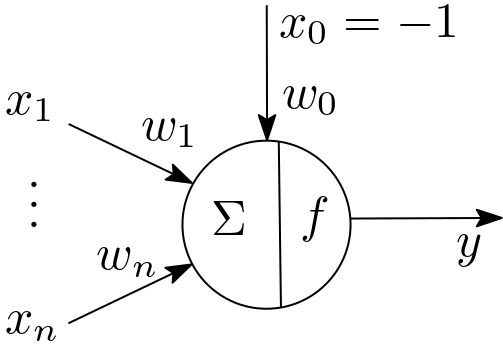
\includegraphics[width=.5\textwidth]{./img/neuronio.png}
\caption{Modelo abstrato de um neurônio artificial. Fonte: \cite{Teresa:Livro}.}
\label{fig:neuronio}
\end{figure}

O poder computacional de um neurônio individual é limitado às funções linearmente separáveis. Ao dispor os neurônios em camadas e conectá-los a todos os neurônios da camada seguinte, conforme estabelecido nas RNAs MLP, torna-se possível uma transformação sucessiva nos dados de entrada que os tornam linearmente separáveis à medida que se aproximam da camada de saída \cite{Faceli:Livro}, conforme ilustrado na Figura \ref{fig:mlp}.

\begin{figure}[ht]
\centering
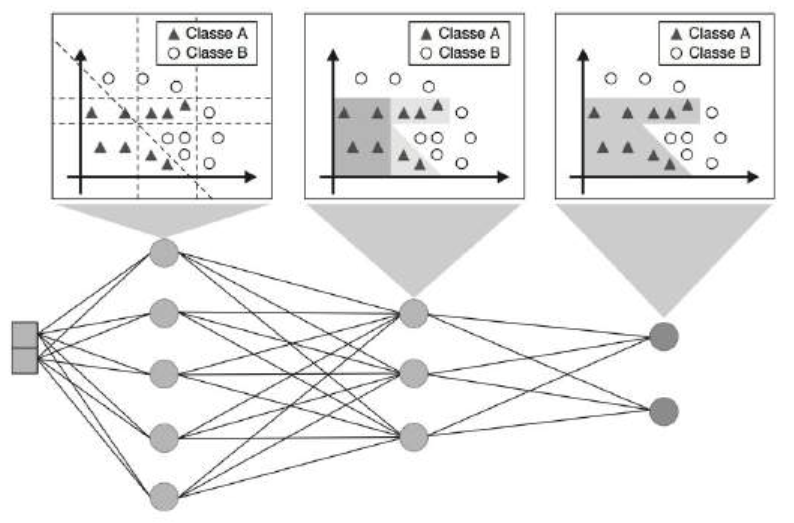
\includegraphics[width=.8\textwidth]{./img/mlp.png}
\caption{Papel desempenhado pelos neurônios em cada camada de uma RNA MLP. Fonte: \cite{Faceli:Livro}.}
\label{fig:mlp}
\end{figure}

O aprendizado das RNAs se dá por meio de um processo iterativo de ajustes aplicado a seus pesos, fazendo com que o modelo obtenha melhor desempenho, normalmente medido pela acurácia preditiva. Esses algoritmos, são formados por um conjunto de regras bem definidas que determinam quando e como dever ser alterado o valor de cada peso \cite{Faceli:Livro}. Um método popular para o aprendizado supervisionado de MLPs é o algoritmo de \emph{backpropagation}, que consiste em duas fases: uma fase pra frente (\emph{forward}) e outra pra trás (\emph{backwards}). Na fase \emph{forward}, os pesos sinápticos da rede são fixos e o sinal de entrada é propagado pela rede, camada por camada, até atingir a saída. Na segunda fase \emph{backwards}, um sinal de erro é produzido comparando a saída da rede com uma resposta desejada. O sinal de erro resultante é propagado através da rede, camada por camada, porém a propagação é realizada pra trás \cite{Faceli:Livro,Haykin:NeuralNetworksBook}. Nesta segunda fase, ajustes sucessivos são feitos nos pesos da rede utilizando o algoritmo do gradiente descendente \cite{Teresa:Livro}.

As CNNs são uma categoria de RNAs especialmente voltadas para lidar com dados de alta dimensionalidade, tais como imagens, áudio, vídeo, etc. Elas operam de maneira muito semelhante às RNAs MLP, mas com uma diferenças fundamentais no tocante aos neurônios e aos tipos de camada. Os neurônios artificiais convolucionais são caracterizados por um filtro que é convoluído com a entrada, permitindo uma extração apropriada de características frente ao tipo de dado de entrada, pois são capazes de abstrair características como texturas, contornos, cores, etc. As camadas compostas de neurônios convolucionais são chamadas de camadas convolucionais \cite{Khan:2018}.

As CNNs também fazem uso de camadas de \emph{pooling}, tipicamente dispostas após as camadas convolucionais, com vistas a promover uma redução de dimensionalidade, produzindo representações condensadas das entradas. As diversas camadas convolucionais e de \emph{pooling} na arquitetura de uma CNN são responsáveis pela extração automática de características da entrada, as quais passam por camadas densas, tipicamente dispostas ao final da CNN, com vistas a produzir a saída desejada para a tarefa em questão (classificação, regressão, etc.) \cite{Buduma:2018,Chollet:2017}.

Como a extração de características nas CNNs é automática e massiva, é importante utilizar alguma estratégia para descartar valores que podem estar associados à ruído ou que possuem pouca influência na saída do modelo. Isso é feito com camadas de \emph{Dropout}, as quais são compostas de neurônios com limiar para descartar aleatoriamente certas conexões ao longo do treino, colaborando para a regularização e para a diminuição no número de parâmetros ajustáveis das CNNs \cite{Buduma:2018,Chollet:2017}.

As CNNs são tipicamente utilizadas perante o paradigma de Aprendizado Supervisionado com especial destaque para tarefas de classificação em Visão Computacional, representando o estado da arte em diversos problemas nesse domínio \cite{Khan:2018}. Citam-se algumas arquiteturas canônicas de CNNs, tais como, LeNet, AlexNet, Inception e VGG-16, as quais obtiveram desempenho notável em diversas edições do \emph{ImageNet Large Scale Visual Recognition Challenge} (LSVRC) \cite{ILSVRC15}.
